\documentclass[twocolumn]{aastex63}

% typography
\usepackage[T1]{fontenc}

\setlength{\parindent}{1.\baselineskip}
\newcommand{\acronym}[1]{{\small{#1}}}
\newcommand{\package}[1]{\textsl{#1}}
\newcommand{\gaia}{\textsl{Gaia}}
% \newcommand{\hst}{\textsl{HST}}
% \newcommand{\pans}{\textsl{Pan-STARRS}}

% \newcommand{\deg}{\ensuremath{\textrm{deg}}}
\newcommand{\msun}{\ensuremath{\textrm{M}_\odot}}
\newcommand{\myr}{\ensuremath{\textrm{Myr}}}
\newcommand{\gyr}{\ensuremath{\textrm{Gyr}}}
\newcommand{\kpc}{\ensuremath{\textrm{kpc}}}
\newcommand{\kms}{\ensuremath{\textrm{km}\,\textrm{s}^{-1}}}
\newcommand{\masyr}{\ensuremath{\textrm{mas}\,\textrm{yr}^{-1}}}
\newcommand{\feh}{\ensuremath{\textrm{[Fe/H]}}}
\newcommand{\afe}{\ensuremath{\textrm{[$\alpha$/Fe]}}}
\newcommand{\changes}[1]{{\textbf{#1}}}
\hyphenation{kruijs-sen}

% aastex parameters
% \received{not yet; THIS IS A DRAFT}
%\revised{not yet}
%\accepted{not yet}
% % Adds "Submitted to " the argument.
% \submitjournal{ApJ}
\shorttitle{}
\shortauthors{bonaca \& kruijssen}

%@arxiver{}
\usepackage{amsmath}

\begin{document}\sloppy\sloppypar\raggedbottom\frenchspacing % trust me

\title{The low masses of globular clusters dissolved in the Milky Way}

\correspondingauthor{Ana~Bonaca}
\email{ana.bonaca@cfa.harvard.edu}

\author[0000-0002-7846-9787]{Ana~Bonaca}
\affil{Center for Astrophysics | Harvard \& Smithsonian, 60 Garden Street, Cambridge, MA 02138, USA}

\author[0000-0002-8804-0212]{J.~M.~Diederik~Kruijssen}
\affiliation{Astronomisches Rechen-Institut, Zentrum f\" ur Astronomie der Universit\" at Heidelberg, M\" onchhofstra\ss e 12-14, D-69120 Heidelberg, Germany}
\affil{Center for Astrophysics | Harvard \& Smithsonian, 60 Garden Street, Cambridge, MA 02138, USA}


\begin{abstract}\noindent % trust me
Numerous stellar streams that have been discovered in the Milky Way as evaporated globular clusters show signs of dynamical perturbation.
N-body models that can illuminate the origin of these perturbations require the cluster's initial mass as a fundamental input parameter.
Here we present orbits and masses of 20 dissolved globular clusters in the Milky Way.
We constrained the streams' orbits by fitting the 3D positions of a stream's endpoints from ground-based photometry and its proper motions from Gaia.
Assuming a dissolution time of 10\,Gyr, we use orbital apocenters and eccentricities to estimate the clusters' initial mass.
Disrupted globular clusters have preferentially lower masses than the surviving population, with the median mass being an order of magnitude smaller.
The overall distribution of apocenters and eccentricities is similar for the disrupted and surviving clusters, however, at a fixed mass disrupted clusters have smaller apocenters and larger eccentricities.
The progenitors of tidal streams observed at the present are a specific, low-mass subset of the initial globular cluster population.
This has implications for establishing the role of internal dynamics in sculpting the observed tidal debris, and the amount of external perturbation, e.g., from dark-matter subhalos, that these streams experienced.
% modeling how much the tidal streams were shaped by nature versus nurture.
% 
% - GCs individually: birth sites of binary black holes, some of the oldest stars in the universe
% - collectively: tracers of dark matter halo mass, accretion history
% - mass basic property, but have biased view, bc some tidally disrupted
% - implications for: gc formation mechanisms? 
\end{abstract}

\section{Introduction}
\label{sec:intro}


\section{Stream Orbits}
\label{sec:orbits}
A total of x thin stellar streams, likely disrupted globular clusters, have been reported in the Milky Way \citep[an up-to-date list is available in the \package{galstreams} package,][]{mateu:2018}.
Tidal debris from evaporating globular clusters nearly delineates the progenitor's orbit \citep[e.g.,][]{kupper:2012}, however, kinematic information is essential for accurate stream modeling \citep{bh:2018}.
Here we analyze a subset of y stellar streams with published proper motions (Table~\ref{table:streams}).

We measure orbital parameters for a population of dissolved globular clusters by fitting orbits to sky positions, distances, and proper motions of stream endpoints.
Due to limited observational data on some streams, we decided to fit only the stream endpoints to ensure a homogeneous treatment of the entire sample.
\citet{riley:2020} demonstrated that the 3D positions of stream end-points robustly constrain their orbital poles, while \citet{ibata:2019} found that the absence of radial velocities produces no significant biases in orbit determination for streams with proper motion data.
Therefore, we expect our strategy of recovering orbits from 5D positions of stream endpoints to perform well.
In Section~\ref{sec:discussion} we discuss how orbital constraints change for streams where additional data is available.
The endpoint sky positions and distances \citep{riley:2020}, and proper motions \citep[][as noted]{ibata:2019, shipp:2019} are listed in Table~\ref{table:streams}, along with the associated uncertainties.
Figure~\ref{fig:streams} shows these data for three representative streams as large black points (top to bottom: x, y, z).

We fit stream orbits in a three-component model of the Milky Way gravitational potential implemented in the \package{gala} package \citep{gala} and featuring a \citet{mn:1975} disk (mass: $5.5\times10^{10}\rm\, M_\odot$, scale-length: 3\,kpc, scale-height: 28\,pc), a \citet{hernquist:1990} bulge (mass: $4\times10^9\rm\, M_\odot$, scale-radius: 1\,kpc), and a \citet{nfw:1997} halo (scale-mass: $7\times10^{11}\rm\, M_\odot$, scale-radius: 15.62\,kpc, $z$-axis flattening: 0.95).
Similar to the orbit-fitting procedure of \citet{pwb}, we represent the orbit as a 6D location in phase-space, fixing its right ascension, R.A., and solving for the remaining 5D coordinates (declination, distance, radial velocity, two proper motion components).
At the R.A. of the stream endpoints, we evaluate the orbital declinations, distances and proper motions against the observations, assuming Gaussian uncertainties.
The orbits are initialized at one of the stream endpoints, with a radial velocity such that the total velocity vector equals the circular velocity at that Galactocentric distance and points to the other endpoint.
We employ only minimal priors by requiring a bound orbit and the absolute radial velocity lower than 500\,\kms.

We begin the search for well-fitting stream orbits by maximizing the likelihood of orbits passing through the observed endpoints using the \package{scipy} implementation of the BFGS algorithm.
Starting with this best-fitting solution, we further sample the likelihood with an affine-invariant sampler \package{emcee} to estimate the posterior distribution of the orbital parameters.
We advanced 64 walkers for 512 steps and kept the last 256 steps which converged to constant median and dispersion values for all model parameters.
The median, 16th and 84th percentiles of the constrained 5D coordinates are reported for each stream's orbit in Table~\ref{table:constraints}.
- results in figure: lines samples from the posterior, also colored by distance
- zoom in: track fit very well, orbit fits expect some distance gradients, can be improved in the future w better selected members

- used these to integrate orbit x Gyr (on avg y periods) and estimate the orbital apocenter, $R_{apo}$, and eccentricity, $e=(R_{apo} - R_{peri})/(R_{apo} + R_{peri})$.
- samples shown in next figure, spread in peri, apo
- to account for these covariances, but keep runtime manageable, we calculated orbits using 1000 random samples from the posterior \footnote{available at the project repository \url{https://github.com/abonaca/disrupted_gc}}, and report the median, 16th and 84th percentiles of the orbital apocenter and eccentricity in Table~\ref{table:constraints}.

% In addition, we stored 1000 random posterior samples \footnote{available at the project repository \url{https://github.com/abonaca/disrupted_gc}} and used them to estimate the orbital eccentricity, pericenter
% estimate propagate parameter covariances into orbital parameters and cluster masses

% - orbit xGyr in the future, on average y orbital periods, that we use to measure apocenter $R_{apo}$, eccentricity, $e=(R_{apo} - R_{peri})/(R_{apo} + R_{peri})$
% - within one orbit peri/apo precisely measured (fractional precision x), across samples, median/90 percentile fractional uncertainty for apocenter, eccentricity
% - two examples: different kinds of orbits, same precision?


\section{Masses of Disrupted GCs}
\label{sec:disrupted}

We estimate the masses of the GCs producing the streams using a simple analytic GC disruption model \citep{lamers05}, which reproduces direct $N$-body simulations of GCs undergoing tidal evaporation in a static background potential \citep{baumgardt03}. Specifically, we obtain a `pre-evaporation' GC mass $M_0$ by estimating the total mass loss due to stellar evolution and tidal evaporation for a cluster on the inferred orbit over some timescale $t$. We refrain from deriving an `initial' GC mass, because tidal evaporation in the host galaxy halo is not the only mass loss mechanism experienced by GCs over the course of their history. Prior to being deposited into the halo, GCs were disrupted by tidal shocks due to gravitational perturbations from overdensities in the interstellar medium of their natal galaxy \citep[e.g.][]{gieles06,kruijssen11,miholics17,pfeffer18}. Integrated over the history of GCs, tidal shocks are thought to dominate the total dynamical mass loss \citep[e.g.][]{kruijssen15b}. Therefore, the quantity $M_0$ refers strictly to the `pre-evaporation' GC mass -- after the first phase of disruption tidal shocks, but before the second phase of disruption by tidal evaporation. We also include the total amount of mass lost by stellar evolution, so that only the mass loss by tidal shocks is unaccounted for.

We relate $M_0$ to the orbit of the stellar stream by assuming a present-day GC mass of zero (consistent with the fact that only a fossil stream remains) and writing eq.~7 of \citet{lamers05} as
\begin{equation}
\label{eq:m0}
M_{\rm 0}=\frac{1}{\mu_{\rm ev}(t)}\left(\frac{\gamma t}{t_0}\right)^{1/\gamma} .
\end{equation}
In this expression, $\mu_{\rm ev}(t)$ is the fraction of the initial GC mass lost by stellar evolution, provided by \citet{lamers05} as
\begin{equation}
\label{eq:muev}
\mu_{\rm ev}(t)=1-q_{\rm ev} ,
\end{equation}
with
\begin{equation}
\label{eq:qev}
\log_{10}{q_{\rm ev}}(t) = [\log_{10}(t/{\rm yr})-a_{\rm ev}]^{b_{\rm ev}}+c_{\rm ev} ,
\end{equation}
and $a_{\rm ev} = 6.93$, $b_{\rm ev} = 0.255$, and $c_{\rm ev} = -1.682$, appropriate for a GC-like metallicity of $0.02{\rm Z}_\odot$ and a \citet{kroupa01} stellar initial mass function \citep{kruijssen08}. The variables $\gamma$ and $t_0$ represent the exponent and proportionality factor, respectively, of the Lamers cluster disruption law:
\begin{equation}
\label{eq:lamers}
\tau_{\rm dis}=t_0\left(\frac{M}{\msun}\right)^\gamma ,
\end{equation}
where $\tau_{\rm dis}$ is the cluster disruption timescale. We follow \citet{kruijssen09} in adopting $\gamma=0.7$ and relating $t_0$ to the orbital parameters as
\begin{equation}
\label{eq:t0}
t_0 = t_{0,\odot}\left(\frac{R_{\rm a}}{8.5~\kpc}\right)\left(\frac{v_{\rm c}}{220~\kms}\right)^{-1}(1-e) ,
\end{equation}
with $t_{0,\odot}=10.7~\myr$ and $R_{\rm a}$, $v_{\rm c}$, and $e$ denoting the orbital apocenter radius, circular velocity, and orbital eccentricity, respectively. Finally, we assume that the time spent by each GC orbiting the Milky Way prior to dissolving into a fossil stream is $t=10~\gyr$. This is motivated by the typical ages of GCs in the Galactic halo \citep[$\sim12~\gyr$, e.g.][]{kruijssen19e} and by recent results showing that fossil stream lifetimes are much shorter than GC ages (!!REF), such that the progenitors of fossil streams must have disrupted in the past few Gyr. Our results are robust to this choice -- an error of 0.3~dex (i.e.\ a factor of 2) in $t$ translates into an error of just 0.2~dex in the pre-evaporation mass $M_0$.

\begin{figure*}
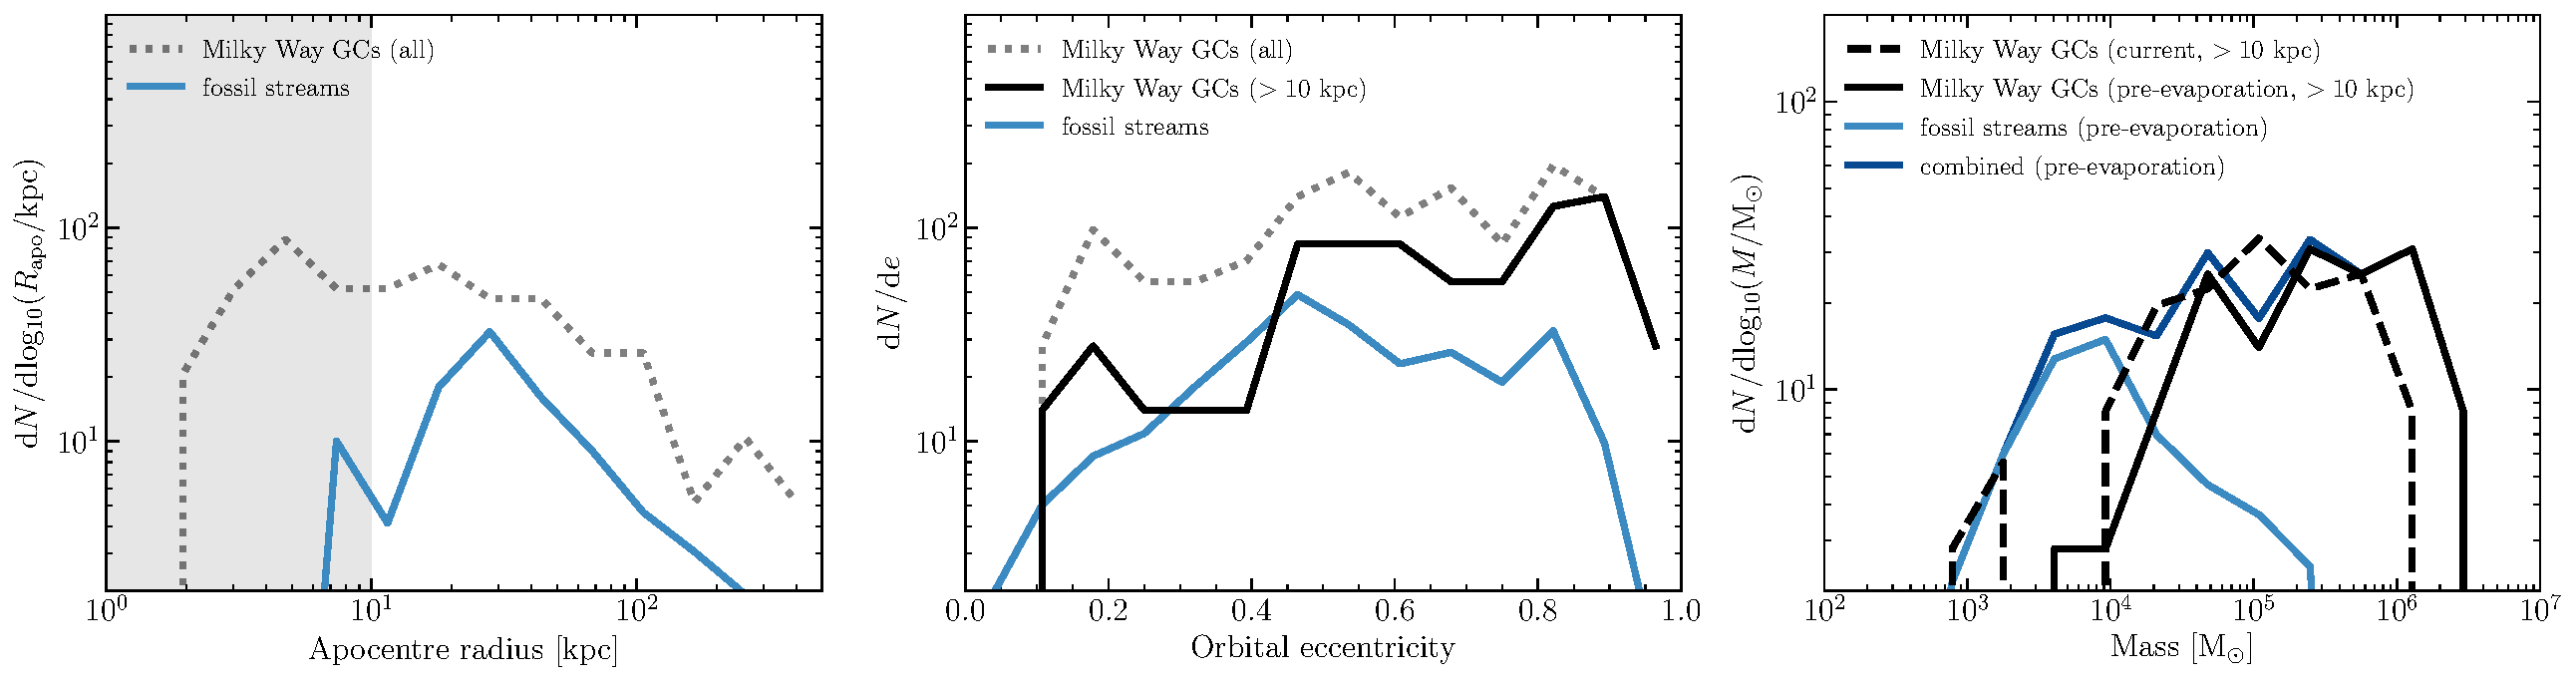
\includegraphics[width=\hsize]{figures/distributions_mc.pdf}%
\caption{
\label{fig:hist}
Caption text.}
\end{figure*}	
We propagate the uncertainties on the fossil streams' orbital parameters into those on the pre-evaporation masses by applying eq.~(\ref{eq:m0}) to the entire sample of MCMC solutions. The resulting distributions of all apocenter radii, eccentricities, and pre-evaporation masses of the fossil streams in the MCMC sample are shown in \autoref{fig:hist}, where we also include the population statistics of Galactic GCs that have survived till the present day. For these surviving GCs, we also include an estimate of their pre-evaporation masses.


\section{Discussion}
\label{sec:discussion}
- summary

- caveats:
-- orbit fits -> compare to published ones; 5d fits predictive, don't change much w 6d (ibata)
-- stream ne orbit
-- 10 Gyr disruption time for estimating the mass

% - check how sensitive the inferred rapo is on the details of the stream track used
% - for streams w published

- compare to mass estimates in the detect part of the stream -> are they mostly detected or are they extending past the currently detected endpoints?

- lower mass -> implications for epicycles

\vspace{0.5cm}
It is a pleasure to thank:

\software{
\package{Astropy} \citep{astropy, astropy:2018},
\package{gala} \citep{gala},
\package{IPython} \citep{ipython},
\package{matplotlib} \citep{mpl},
\package{numpy} \citep{numpy},
\package{scipy} \citep{scipy}
}

\bibliographystyle{aasjournal}
\bibliography{disrupted_gc}


\end{document}


